\documentclass{report}
\usepackage{graphicx, tikz-cd, float, titlepic, booktabs} % Required for inserting images
\usepackage{pgfplots}
\usepackage{multicol}
\usepackage{makecell}
\pgfplotsset{compat=1.15}
\usepackage{mathrsfs}
\usetikzlibrary{arrows}
\usepackage{amsmath, amssymb, amsthm, amsfonts, siunitx, physics, gensymb}
\AtBeginDocument{\RenewCommandCopy\qty\SI}
\usepackage[version=4]{mhchem}
\usepackage[most,many,breakable]{tcolorbox}
\usepackage{xcolor, fancyhdr, varwidth}
\usepackage[Glenn]{fncychap}
%Options: Sonny, Lenny, Glenn, Conny, Rejne, Bjarne, Bjornstrup
\usepackage{hyperref, cleveref}
\usepackage{icomma, enumitem} %comma as decimal and continue enumerate with [resume]
\usepackage{plimsoll} %use standard state symbol with \stst
\usepackage[danish]{babel}
\renewcommand{\cellalign}{cl}
\renewcommand{\theadalign}{cl}
\renewcommand\theadfont{\bfseries}
%%%%%%%%%%%%%%%%%%%%%%%%%%%%%%
% SELF MADE COLORS
%%%%%%%%%%%%%%%%%%%%%%%%%%%%%%
\definecolor{myg}{RGB}{56, 140, 70}
\definecolor{myb}{RGB}{45, 111, 177}
\definecolor{myr}{RGB}{199, 68, 64}
\definecolor{mytheorembg}{HTML}{F2F2F9}
\definecolor{mytheoremfr}{HTML}{00007B}
\definecolor{mylenmabg}{HTML}{FFFAF8}
\definecolor{mylenmafr}{HTML}{983b0f}
\definecolor{mypropbg}{HTML}{f2fbfc}
\definecolor{mypropfr}{HTML}{191971}
\definecolor{myexamplebg}{HTML}{F2FBF8}
\definecolor{myexamplefr}{HTML}{88D6D1}
\definecolor{myexampleti}{HTML}{2A7F7F}
\definecolor{mydefinitbg}{HTML}{E5E5FF}
\definecolor{mydefinitfr}{HTML}{3F3FA3}
\definecolor{notesgreen}{RGB}{0,162,0}
\definecolor{myp}{RGB}{197, 92, 212}
\definecolor{mygr}{HTML}{2C3338}
\definecolor{myred}{RGB}{127,0,0}
\definecolor{myyellow}{RGB}{169,121,69}
\definecolor{myexercisebg}{HTML}{F2FBF8}
\definecolor{myexercisefg}{HTML}{88D6D1}
%%%%%%%%%%%%%%%%%%%%%%%%%%%%%%%%%%%%%%%%%%%%%%%%%%%%%%%%%%%%%%%%%%%%%%
% Box environments for theorems and problems
%%%%%%%%%%%%%%%%%%%%%%%%%%%%%%%%%%%%%%%%%%%%%%%%%%%%%%%%%%%%%%%%%%%%%
\setlength{\parindent}{1cm}
%================================
% Question BOX
%================================
\makeatletter
\newtcbtheorem{question}{Opgave}{enhanced,
	breakable,
	colback=white,
	colframe=myb!80!black,
	attach boxed title to top left={yshift*=-\tcboxedtitleheight},
	fonttitle=\bfseries,
	title={#2},
	boxed title size=title,
	boxed title style={%
			sharp corners,
			rounded corners=northwest,
			colback=tcbcolframe,
			boxrule=0pt,
		},
	underlay boxed title={%
			\path[fill=tcbcolframe] (title.south west)--(title.south east)
			to[out=0, in=180] ([xshift=5mm]title.east)--
			(title.center-|frame.east)
			[rounded corners=\kvtcb@arc] |-
			(frame.north) -| cycle;
		},
	#1
}{def}
\makeatother
%================================
% DEFINITION BOX
%================================

\newtcbtheorem[number within=section]{definition}{Definition}{enhanced,
	before skip=2mm,after skip=2mm, colback=red!5,colframe=red!80!black,boxrule=0.5mm,
	attach boxed title to top left={xshift=1cm,yshift*=1mm-\tcboxedtitleheight}, varwidth boxed title*=-3cm,
	boxed title style={frame code={
					\path[fill=tcbcolback]
					([yshift=-1mm,xshift=-1mm]frame.north west)
					arc[start angle=0,end angle=180,radius=1mm]
					([yshift=-1mm,xshift=1mm]frame.north east)
					arc[start angle=180,end angle=0,radius=1mm];
					\path[left color=tcbcolback!60!black,right color=tcbcolback!60!black,
						middle color=tcbcolback!80!black]
					([xshift=-2mm]frame.north west) -- ([xshift=2mm]frame.north east)
					[rounded corners=1mm]-- ([xshift=1mm,yshift=-1mm]frame.north east)
					-- (frame.south east) -- (frame.south west)
					-- ([xshift=-1mm,yshift=-1mm]frame.north west)
					[sharp corners]-- cycle;
				},interior engine=empty,
		},
	fonttitle=\bfseries,
	title={#2},#1}{def}

%================================
% NOTE BOX
%================================

\usetikzlibrary{arrows,calc,shadows.blur}
\tcbuselibrary{skins}
\newtcolorbox{note}[1][]{%
	enhanced jigsaw,
	colback=gray!20!white,%
	colframe=gray!80!black,
	size=small,
	boxrule=1pt,
	title=\textbf{Note:},
	halign title=flush center,
	coltitle=black,
	breakable,
	drop shadow=black!50!white,
	attach boxed title to top left={xshift=1cm,yshift=-\tcboxedtitleheight/2,yshifttext=-\tcboxedtitleheight/2},
	minipage boxed title=1.5cm,
	boxed title style={%
			colback=white,
			size=fbox,
			boxrule=1pt,
			boxsep=2pt,
			underlay={%
					\coordinate (dotA) at ($(interior.west) + (-0.5pt,0)$);
					\coordinate (dotB) at ($(interior.east) + (0.5pt,0)$);
					\begin{scope}
						\clip (interior.north west) rectangle ([xshift=3ex]interior.east);
						\filldraw [white, blur shadow={shadow opacity=60, shadow yshift=-.75ex}, rounded corners=2pt] (interior.north west) rectangle (interior.south east);
					\end{scope}
					\begin{scope}[gray!80!black]
						\fill (dotA) circle (2pt);
						\fill (dotB) circle (2pt);
					\end{scope}
				},
		},
	#1,
}
%================================
% EXAMPLE BOX
%================================
\newtcbtheorem[number within=section, use counter from=definition]{Example}{Example}
{%
	colback = myexamplebg
	,breakable
	,colframe = myexamplefr
	,coltitle = myexampleti
	,boxrule = 1pt
	,sharp corners
	,detach title
	,before upper=\tcbtitle\par\smallskip
	,fonttitle = \bfseries
	,description font = \mdseries
	,separator sign none
	,description delimiters parenthesis
}
{ex}
%================================
% THEOREM BOX
%================================

\tcbuselibrary{theorems,skins,hooks}
\newtcbtheorem[number within=section, use counter from=definition]{Theorem}{Theorem}
{%
	enhanced,
	breakable,
	colback = mytheorembg,
	frame hidden,
	boxrule = 0sp,
	borderline west = {2pt}{0pt}{mytheoremfr},
	sharp corners,
	detach title,
	before upper = \tcbtitle\par\smallskip,
	coltitle = mytheoremfr,
	fonttitle = \bfseries\sffamily,
	description font = \mdseries,
	separator sign none,
	segmentation style={solid, mytheoremfr},
}
{th}

%%%%%%%%%%%%%%%%%%%%%%%%%%%%%%%%%%%%%%%%%%%%%%%%%%%%%%%%%%%%%%%%%
% SELF MADE COMMANDS
%%%%%%%%%%%%%%%%%%%%%%%%%%%%%%
\newcommand{\sol}{\setlength{\parindent}{0cm}\textbf{\textit{Løsning:}}\setlength{\parindent}{1cm}}
%%%%%%%%%%%%%%%%%%%%%%%%%%%%%%%%%
\usepackage[tmargin=2cm,rmargin=1in,lmargin=1in,margin=0.85in,bmargin=2cm,footskip=.2in]{geometry}\pagestyle{fancy}
\lhead{Minrui Kevin Zhou 3.b}
\rhead{H9}

\title{H9\\
{\Large \textbf{3.b fysik A}}}
\author{Kevin Zhou}
\date{\today}

\begin{document}
\maketitle
\begin{question}{Laserkirurgi}{}
En laser, der bruges ved kirurgiske indgreb, virker som en kniv, når laserstrålens energi absorberes af vævet og får det til at fordampe. Laseren udsender fortoner med bølgelængden $10,6 \;\unit{\micro m} $.
\begin{itemize}
  \item[a.] Beregn energien af hver af de udsendte fotoner
\end{itemize}
Laserstrålen afsætter energi i vævet med effekten 60 W. Laserstrålen har en diameter på 0,40 mm og den flyttes hen over vævet med farten 2,0 cm/s. Ved legemstemperatur skal vævet tilføres 2,4 kJ pr gram for at fordampe. Vævets densitet er 0,95 g/cm$^3.$
\begin{itemize}
  \item[b.] Beregn hvor dybt laserstrålen skærer i vævet. Gør herunder rede for de relevante antagelser.
\end{itemize}
\end{question}
\sol \\
\textbf{a.}
Da fotonerne har lysets fart, så må de hver have energien 
\begin{equation*}
\begin{split}
E_{\text{fot} }&=\frac{h \cdot c}{\lambda }\\
&=\frac{6,6261 \cdot 10 ^{-34}\;\unit{J \cdot s} \cdot 3,00 \cdot 10 ^{8} \;\unit{m/s} }{10,6 \cdot 10 ^{-6} \;\unit{m} }\\
&\approx 1,88 \cdot 10 ^{-20} \;\unit{J} \\
&\approx 0,117 \;\unit{eV} 
\end{split}
\end{equation*}
Energien af hver af de udsendte fotoner er altså $1,88 \cdot 10 ^{-20} \;\unit{J} $, hvilket svarer til $0,117 \;\unit{eV} $.\\[1ex]
\textbf{b.}
Vi antager, at energien er fordelt ligeligt på arealet, hvor laserstrålen er på vævet.
Derudover antager vi, at laserstrålen har form som en cirkelskive og bevæger sig med konstant fart i en lige linje.
Fra disse antagelser har vi så, at den maksimale tid, som laseren er på et bestemt punkt må være
\begin{equation*}
\begin{split}
t=\frac{d}{v}
\end{split}
\end{equation*}
hvor $d$ er laserstrålens diameter, og $v$ er laserens fart hen over vævet. 
Et udtryk for energien ville da være
\begin{equation*}
\begin{split}
E=P \cdot t = P \cdot \frac{d}{v}
\end{split}
\end{equation*}
hvor $P$ er effekten, hvormed laseren afsætter energi i vævet. 
Siden vi har ladet laserstrålen have form som en cirkelskive, så må arealet som laserstrålen er på vævet til ethvert tidspunkt være
\begin{equation*}
\begin{split}
A= \pi \cdot r^2 = \pi \cdot \left(\frac{d}{2}\right)^2
\end{split}
\end{equation*}
Den dybde, som laserstrålen skærer i vævet betegner vi $y$.
Siden det tager 2,4 kJ at fordampe $1 \;\unit{g} $ væv, så har vi, at 
\begin{equation*}
\begin{split}
\frac{E}{m}=2,4 \;\unit{kJ/g} &\iff m=\frac{E}{2,4 \;\unit{kJ/g} }\\
&\iff y \cdot A \cdot \rho = \frac{E}{2,4 \;\unit{kJ/g} }\\
&\iff y=\frac{E}{2,4 \;\unit{kJ/g} \cdot A \cdot \rho }\\
&\iff y=\frac{P \cdot \frac{d}{v}}{2,4 \;\unit{kJ/g} \cdot \pi \cdot \left(\frac{d}{2}\right)^2 \cdot \rho }
\end{split}
\end{equation*}
Vi indsætter de givne værdier og beregner $y$.
\begin{equation*}
\begin{split}
y&=\frac{P \cdot \frac{d}{v}}{2,4 \;\unit{kJ/g} \cdot \pi \cdot \left(\frac{d}{2}\right)^2 \cdot \rho }\\
&=\frac{60 \;\unit{W} \cdot \frac{0,40 \cdot 10 ^{-3} \;\unit{m} }{2,0 \cdot 10 ^{-2} \;\unit{m/s} }}{2,4 \cdot 10^3 \;\unit{J/g} \cdot \pi \cdot \left(\frac{0,40 \cdot 10 ^{-1} \;\unit{cm} }{2}\right)^2 \cdot 0,95 \;\unit{g/cm^3} }\\
&\approx 0,42 \;\unit{cm} 
\end{split}
\end{equation*}
Laserstrålen skærer altså $0,42 \;\unit{cm} $ dybt i vævet. 

\begin{question}{Tomatsovs}{}
Til en tomatsovs bruges 8 ensartede tomater, der først vejes og så blendes.
Massen af de 8 tomater er $774 \;\unit{g} $ og de har tilsammen volumen på $8,0 \;\unit{dL} $. 
\begin{itemize}
  \item[a.] Bestem densiteten af en tomat.
  \item[b.] Bestem en tilnærmet værdi for den omsatte elektriske energi under opvarmningen. Forklar, hvilke tilnærmelser du gør.
\end{itemize}
Kogepladen fungerer ved, at elektrisk strøm sendes gennem en modstand, der sidder lige under kogepladen.
Selv om forsyningsspændingen til kogepladen er konstant, viser grafen at den omsatte effekt ikke er konstant.
\begin{itemize}
  \item[c.] Forklar, hvorfor den omsatte effekt aftager under opvarmningen.
\end{itemize}
For at lave en tomatsovs opvarmes de blendede tomater fra 25 °C til 100 °C og koger i nogle minutter.
Under tilberedningen tilføres i alt 325 kJ til selve sovsen, og der fordamper 40 g vand.
\begin{itemize}
  \item[d.] Bestem den specifikke varmekapacitet af de blendede tomater.
\end{itemize}
\end{question}
\sol \\
\textbf{a.}
Vi beregner tomats densitet.
\begin{equation*}
\begin{split}
\rho &=\frac{m}{V}\\
&=\frac{774 \;\unit{g} }{8,0 \;\unit{dL} }\\
&=\frac{774 \;\unit{g} }{8,0 \cdot 10^2 \;\unit{cm^3} }\\
&\approx 0,97 \;\unit{g/cm^3} 
\end{split}
\end{equation*}
Densiteten af en tomat er altså $0,97 \;\unit{g/cm^3} $.\\[1ex]
\textbf{b.}
Vi ser, at den omsatte effekt er variabel mht. tiden.
Der gælder, at den omsatte elektriske energi er 
\[
\Delta E = \int_{t_{\text{start} }}^{t_{\text{slut} }} P(t) \,dt 
\] 
hvor $P(t)$ er effekten som funktion af tiden. 
Det svarer til arealet under $(t,P)$-grafen.
Vi finder en tilnærmet værdi ved at tælle antallet af tern under grafen.
\begin{figure}[H]
\begin{center}
  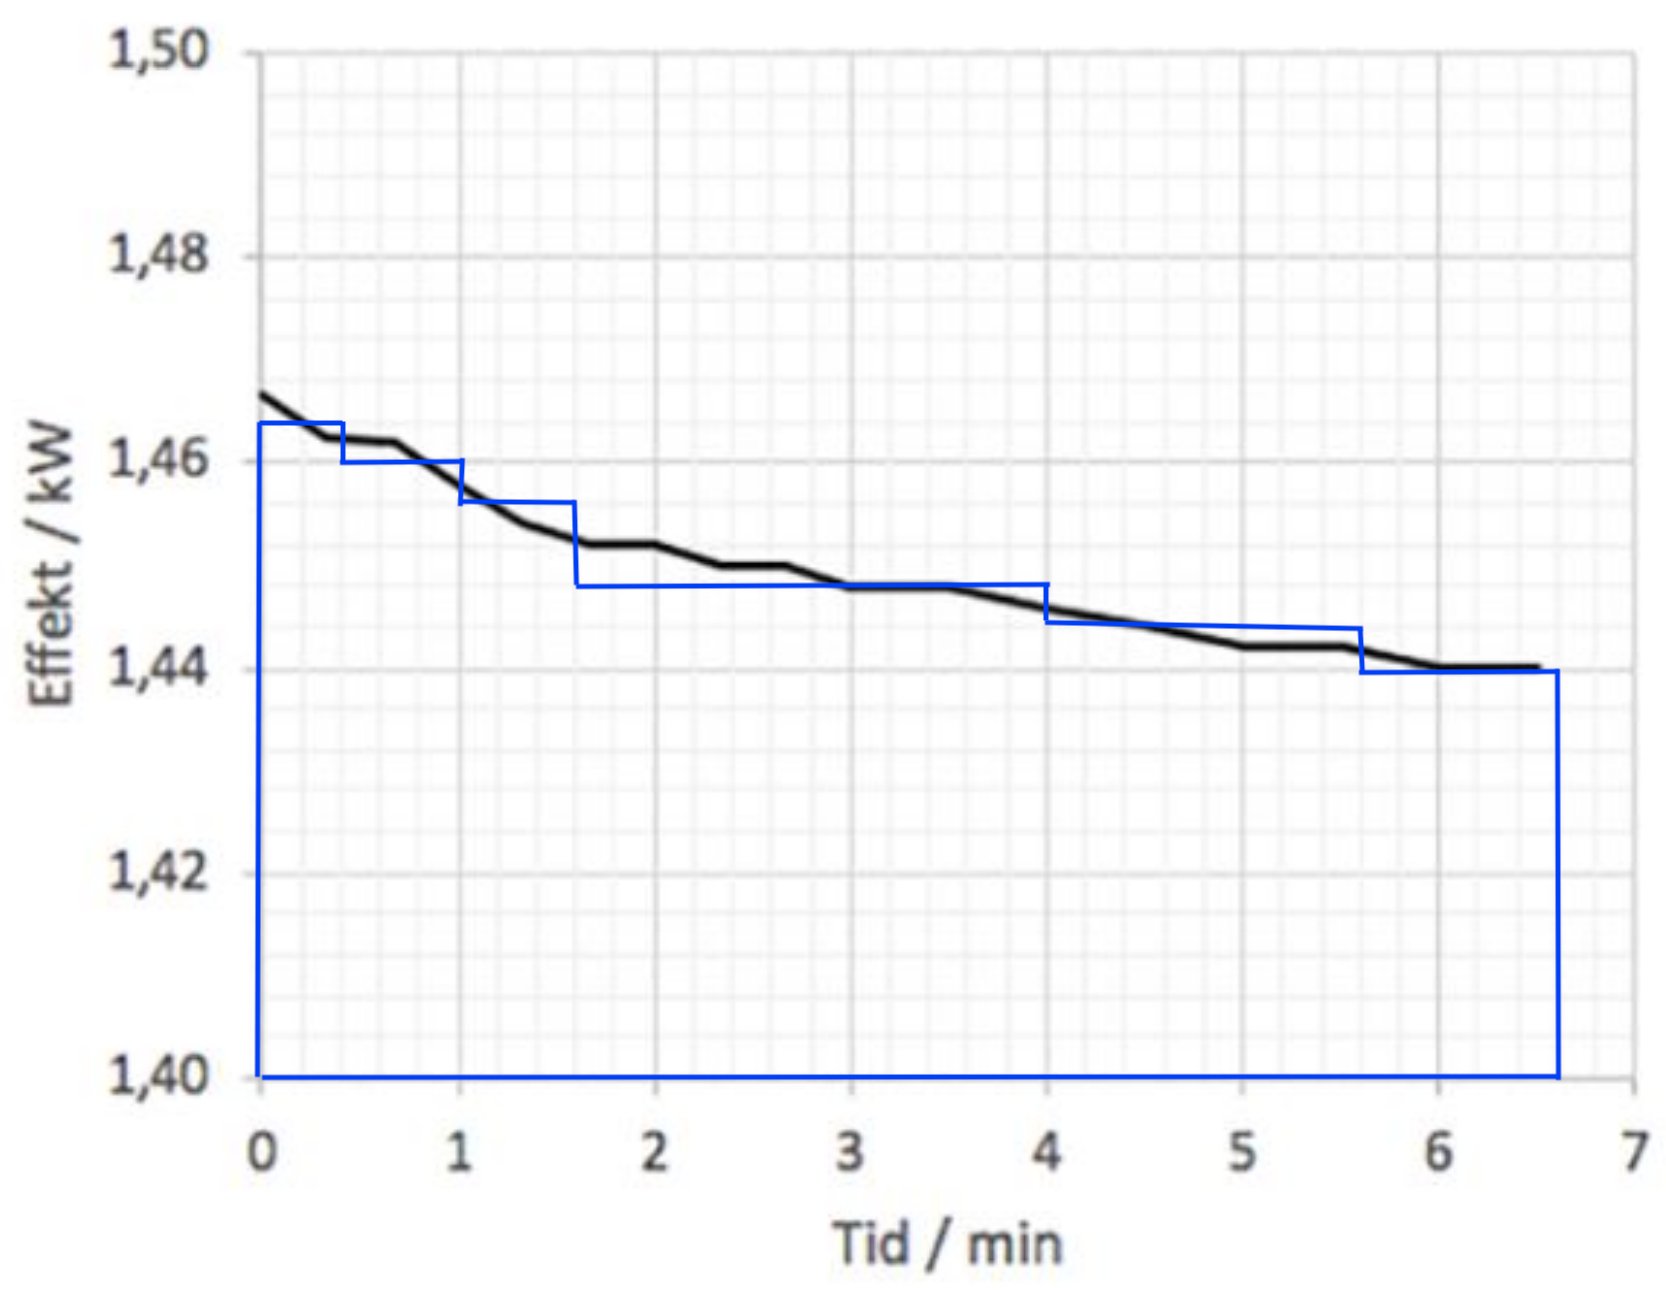
\includegraphics[width=\textwidth]{tern.png}
\end{center}
\caption{Tælning af tern under $(t,P)$-grafen}
\label{fig:tern}
\end{figure}
Hvert lille tern svarer til 
\begin{equation*}
\begin{split}
0,20 \;\unit{min} \cdot \frac{0,02}{5} \;\unit{kW} &=0,20 \cdot 60 \;\unit{s} \cdot \frac{0,02}{5}\;\unit{\frac{kJ}{s}} \\
&=0,048 \;\unit{kJ} 
\end{split}
\end{equation*}
Vi tæller 401 tern under $(t,P)$-grafen i den givne figur, hvilket ses i \cref{fig:tern}.
Det skal dog bemærkes, at $y$-aksen ikke starter fra $0 \;\unit{kW} $, og vi skal derfor lægge $350 \cdot 32,5 =11375$ tern til det talte antal tern. 
Den omsatte elektriske energi må da være
\begin{equation*}
\begin{split}
\Delta E &=(401 + 11375) \cdot 0,048 \;\unit{kJ} \\
&\approx 565 \;\unit{kJ} 
\end{split}
\end{equation*}
En tilnærmet værdi for den omsatte elektriske energi under opvarmningen er altså $565 \;\unit{kJ} $.\\[1ex]
\textbf{c.}
Der gælder for de fleste metaller, at deres resistivitet vokser med temperaturen (jf. Databog s. 182-183).
Der gælder følgende sammenhæng mellem en resistans og resistivitet:
\begin{equation*}
\begin{split}
R=\rho \cdot \frac{l}{A}
\end{split}
\end{equation*}
hvor $\rho $ er resistiviteten, $l$ er ledningens længde, og $A$ er dens tværsnitsareal. 
Siden $l$ og $A$ er konstante for kogepladen, så må resistansen $R$ også vokse, når temperaturen stiger. 
Da der gælder for elektrisk effekt, at 
\begin{equation*}
\begin{split}
P=U \cdot I=\frac{U^2}{R}
\end{split}
\end{equation*}
og der oplyses, at $U$ er konstant, så må $P$ aftage når $R$ vokser, hvilket netop er tilfældet når temperaturen vokser.
Altså vil det sige, at den omsatte effekt aftager, når kogepladen opvarmes.\\[1ex]
\textbf{d.}
Vi antager, at alt den tilførte energi $E$ går til opvarmning af tomatsovsen og fordampning af vandet.
Vi har da
\begin{equation*}
\begin{split}
E=m_{\text{start} } \cdot c _{\text{sovs} } \cdot \Delta T + m _{\text{fordampet} } \cdot L_f (\text{vand}) &\iff c _{\text{sovs} }=\frac{E-m _{\text{fordampet} } \cdot L_f (\text{vand})}{m _{\text{start} } \cdot \Delta T}
\end{split}
\end{equation*}
hvor $L_f(\text{vand} )$ er den specifikke fordampningsvarme for vand, $m _{\text{start} }$ er tomatsovsens masse til start og $m _{\text{fordampet} }$ er massen af den fordampede mængde vand. 
Vi indsætter værdierne og udregner $c _{\text{sovs} }$.
\begin{equation*}
\begin{split}
c _{\text{sovs} }&=\frac{E-m _{\text{fordampet} } \cdot L_f (\text{vand})}{m _{\text{start} } \cdot \Delta T}\\
&=\frac{325 \;\unit{kJ} - 40 \cdot 10 ^{-3} \;\unit{kg} \cdot 2260 \;\unit{kJ/kg} }{774 \cdot 10 ^{-3}\;\unit{kg} \cdot \left(100 \;\unit{\celsius} - 25 \;\unit{\celsius} \right) }\\
&\approx 4,0 \;\unit{\frac{kJ}{kg \cdot \celsius}} \\
&=4,0 \cdot 10^3 \;\unit{\frac{J}{kg \cdot \celsius}} 
\end{split}
\end{equation*}
Den specifikke varmekapacitet af de blendede tomater er altså $4,0 \cdot 10^3 \;\unit{\frac{J}{kg \cdot \celsius}} $.
\begin{question}{3d print}{}
  En komponent med massen 0,157 kg fremstilles af metallegeringen Ti64, som har densiteten $4,40 \cdot 10^3 \;\unit{kg/m^3}$.
  \begin{itemize}
    \item[a.] Beregn rumfanget af komponenten.
  \end{itemize}
Til at smelte metallet anvender man en laser med bølgelængden 1075 nm. Laseren udsender lys med effekten 150 W.
\begin{itemize}
  \item[b.] Hvor mange fotoner udsender laseren pr. sekund?
\end{itemize}
For at fremstille komponenten skal en 3D-printer opvarme og smelte metallegeringen, som komponenten fremstilles af.
Tabellen viser nogle termiske egenskaber for metallegeringen Ti64.
\begin{itemize}
  \item[c.] Vurdér, hvor lang tid det tager laseren at smelte metallegeringen til fremstilling af komponenten.
\end{itemize}
\end{question}
\sol \\
\textbf{a.}
Komponentens volumen er blot dens masse per densitet.
\begin{equation*}
\begin{split}
V&=\frac{m}{\rho }\\
&=\frac{0,157 \;\unit{kg} }{4,40 \cdot 10^3 \;\unit{kg/m^3} }\\
&\approx 3,57 \cdot 10 ^{-5} \;\unit{m^3} \\
&=35,7 \;\unit{cm^3} 
\end{split}
\end{equation*}
Rumfanget af komponenten er altså $35,7 \;\unit{cm^3} $.\\[1ex]
\textbf{b.}
Der gælder, at energien for én foton er 
\[
E _{\text{fot} }=\frac{h \cdot c}{\lambda }
\] 
Lad $n$ være antallet af fotoner, som laseren udskyder.
Så har vi, at den samlede energi fra laserestrålen må være 
\begin{equation*}
\begin{split}
E _{\text{samlet} }= n \cdot E _{\text{fot} } = n \cdot \frac{h \cdot c}{\lambda }
\end{split}
\end{equation*}
Per definition af effekten gælder der
\begin{equation*}
\begin{split}
P=\frac{E _{\text{samlet} }}{t} &\iff P \cdot t = n \cdot \frac{h \cdot c}{\lambda }\\
&\iff n=P \cdot t \cdot \frac{\lambda }{h \cdot c}
\end{split}
\end{equation*}
Vi beregner nu antallet af fotoner, som laseren udsender på ét sekund.
\begin{equation*}
\begin{split}
n&=P \cdot t \cdot \frac{\lambda }{h \cdot c}\\
&=150 \;\unit{W} \cdot 1 \;\unit{s} \cdot \frac{1075 \cdot 10 ^{-9}\;\unit{m} }{6,6261 \cdot 10 ^{-34} \;\unit{J \cdot s} \cdot 3,00 \cdot 10^8 \;\unit{m/s} }\\
&\approx 8,11 \cdot 10^{20}
\end{split}
\end{equation*}
Laseren udsender altså $8,11 \cdot 10 ^{20}$ fotoner hvert sekund. \\[1ex]
\textbf{c.}
Energien, der kræves for at smelte metallegeringen må være
\begin{equation*}
\begin{split}
E&=m \cdot c \cdot \Delta T + m \cdot L_s \\
&=m \cdot \left(c \cdot \Delta T + L_s\right) 
\end{split}
\end{equation*}
Vi kan nu finde et udtryk for tiden, det tager.
\begin{equation*}
\begin{split}
P=\frac{E}{t} &\iff t=\frac{E}{P}\\
&\iff t=\frac{m \cdot \left(c \cdot \Delta T + L_s\right) }{P}
\end{split}
\end{equation*}
Vi antager, at metallegeringen varmes op fra $25 \;\unit{\celsius} $.
Da legeringen skal varmes op til $1660 \;\unit{\celsius} $, så har vi
\[
\Delta T = 1660 \;\unit{\celsius} - 25 \;\unit{\celsius} = 1635 \;\unit{\celsius} 
\] 
Vi udregner nu tiden, det tager at smelte metallegeringen.
\begin{equation*}
\begin{split}
t&=\frac{m \cdot \left(c \cdot \Delta T + L_s\right) }{P}\\
&=\frac{0,157 \;\unit{kg} \cdot \left(0,526 \cdot 10^3 \;\unit{\frac{J}{kg \cdot \celsius}} \cdot 1635 \;\unit{\celsius} + 365 \cdot 10^3\;\unit{J/kg} \right) }{150 \;\unit{W} }\\
&\approx 1,28 \cdot 10^3 \;\unit{s} \\
&=22 \;\unit{min} + 2 \cdot 10 \;\unit{s} 
\end{split}
\end{equation*}
Det tager altså laseren $1,28 \cdot 10^3 \;\unit{s} $ at smelte metallegeringen til komponenten. 
\begin{question}{Galaksen Coma B}{}
  Lyset fra galaksen Coma B undersøges ved at måle på spektret, som indeholder spektrallinjer fra magnesium.
I laboratoriet har en spektrallinje fra magnesium bølgelængden 517,5 nm. Figuren viser et energiniveaudiagram for magnesium med angivelse af grundtilstanden og udvalgte exciterede tilstande.
\begin{itemize}
  \item[a.] Bestem, hvilken overgang i magnesium der giver anledning til emission af lys med bølgelængden 517,5 nm.
\end{itemize}
Når spektrallinjen med bølgelængden 517,5 nm måles i et spektrum fra galaksen Coma B, er den rødforskudt og har bølgelængden 528,6 nm.
\begin{itemize}
  \item[b.] Bestem den nuværende afstand til galaksen Coma B.
\end{itemize}
\end{question}
\sol \\
\textbf{a.}
Vi beregner først energien af en foton med bølgelængden $517,5 \;\unit{nm} $.
\begin{equation*}
\begin{split}
E _{\text{fot} }&=\frac{h \cdot c}{\lambda }\\
&=\frac{6,6261 \cdot 10 ^{-34} \;\unit{J \cdot s} \cdot 3,00 \cdot 10^8 \;\unit{m/s} }{517,5 \cdot 10 ^{-9}\;\unit{m} }\\
&\approx 3,841 \cdot 10 ^{-19} \;\unit{J} \\
&=0,3841 \;\unit{aJ} 
\end{split}
\end{equation*}
Det ses på \cref{fig:energi}, at overgangen fra energiniveau C til energiniveau A er den, som passer bedst mht. forskellen på energierne. 
Vi udregner energien af den exciterede foton
\begin{equation*}
\begin{split}
E _{\text{fot} }&=E_C-E_A\\
&=0,8185 \;\unit{aJ} - 0,4346 \;\unit{aJ} \\
&=0,3839 \;\unit{aJ} 
\end{split}
\end{equation*}
Vi ser, at det passer godt med den udregnede energi for fotoner med bølgelængden $517,5 \;\unit{nm} $.
Altså er det overgangen fra energiniveau C til energinivau A, som giver anledning til emmision af lys med bølgelængden $517,5 \;\unit{nm} $.
\begin{figure}[H]
\begin{center}
  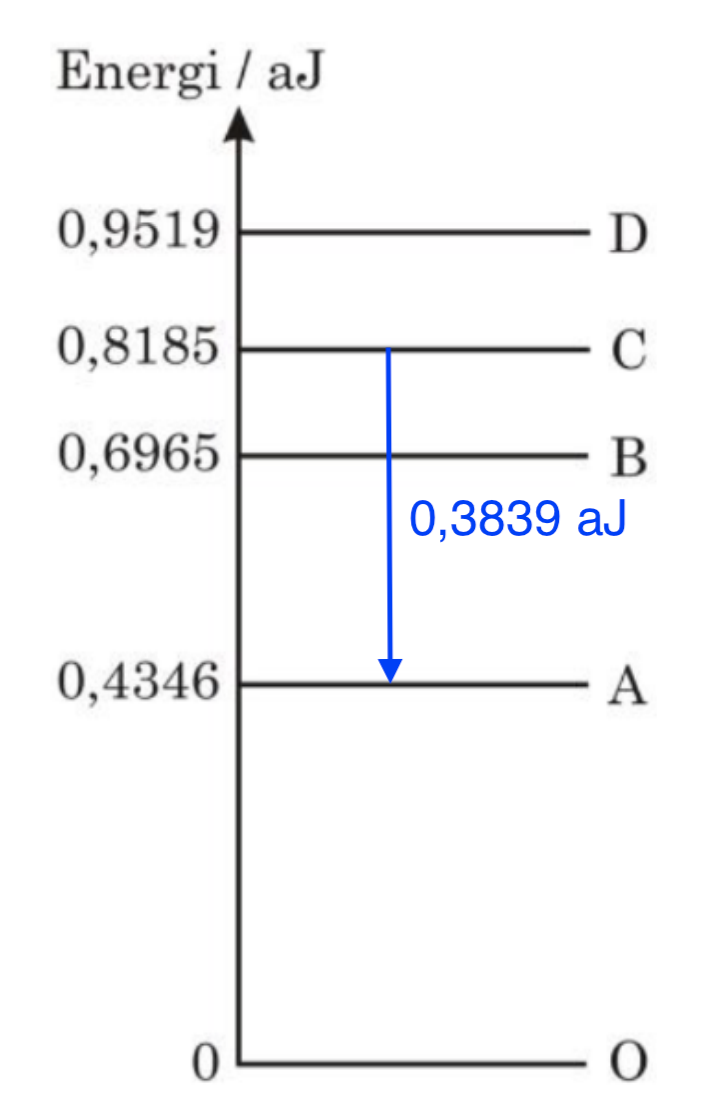
\includegraphics[width=0.3\textwidth]{energi.png}
\end{center}
\caption{Energiniveaudiagram for magnesium}
\label{fig:energi}
\end{figure}
\noindent \textbf{b.}
Der gælder, at galaksens nuværende fart væk fra os er 
\begin{equation*}
\begin{split}
v=c \cdot \frac{\lambda _{\text{obs} }-\lambda _{\text{lab } }}{\lambda _{\text{lab } }}
\end{split}
\end{equation*}
hvor $c$ er lysets fart, $\lambda _{\text{obs} }$ er bølgelængden, der observeres for den givne spektrallinje i spektret og $\lambda _{\text{lab } }$ er bølgelængden for den tilsvarende spektrallinje i laboratoriet. 

Lad $r$ være galaksen nuværende afstand fra os, og lad $H$ være Hubble-konstanten.
Fra Hubbles lov har vi så
\begin{equation*}
\begin{split}
v=H \cdot r &\iff r=\frac{v}{H}\\
&\iff r=c \cdot \frac{\lambda _{\text{obs} }-\lambda _{\text{lab } }}{\lambda _{\text{lab } } \cdot H}
\end{split}
\end{equation*}
Vi beregner nu $r$.
\begin{equation*}
\begin{split}
r&=c \cdot \frac{\lambda _{\text{obs} }-\lambda _{\text{lab } }}{\lambda _{\text{lab } } \cdot H}\\
&=3,00 \cdot 10^8 \;\unit{m/s} \cdot \frac{528,6 \;\unit{nm} -517,5 \;\unit{nm} }{517,5 \;\unit{nm} \cdot 2,3 \cdot 10 ^{-18} \;\unit{s ^{-1}} }\\
&= 2,797732 \cdot 10 ^{24} \;\unit{m} \cdot \frac{1}{9,4607 \cdot 10 ^{15} } \;\unit{\frac{ly}{m}} \\
&\approx 2,957 \cdot 10^8 \;\unit{ly} 
\end{split}
\end{equation*}
Den nuværende afstand til galaksen Coma B er altså $2,957 \cdot 10^8 \;\unit{ly} $.
\begin{question}{Smeltevand fra gletsjer}{}
 Den radioaktive isotop \ce{^35S} anvendes til undersøgelse af smeltevandet fra en gletsjer.
 \begin{itemize}
  \item[a.] Opskriv reaktionsskemaet for det radioaktive henfald af \ce{^35S}.
 \end{itemize}
Forskere undersøger, om smeltevandet kommer fra det seneste års nedbør, eller om det kommer fra de ældre lag af gletsjeren. 
Til en måling opsamles smeltevand, og heri måles aktiviteten fra \ce{^35S} til $0,0055 \;\unit{Bq/kg}$.
Aktiviteten fra \ce{^35S} i nyfalden sne over gletsjeren er $11 \;\unit{Bq/m^3}$. 
Sneens densitet er $240 \;\unit{kg/m^3}$.
\begin{itemize}
  \item[b.] Vurdér, hvor lang tid der er gået, siden det opsamlede smeltevand faldt som sne over gletsjeren. 
\end{itemize}
\end{question}
\sol \\
\textbf{a.}
På kernekortet aflæses det, at \ce{^35_16S} henfalder ved $\beta^-$-henfald.
Vi opskriver reaktionsskemaet for henfaldet.
\begin{equation*}
\begin{split}
\ce{^35_16S -> ^35_17Cl + ^0_-1e + \bar{\nu }} 
\end{split}
\end{equation*}
For god ordens skyld kontrollerer vi, at nukleontallet $A$, ladningen $Z$ og leptontallet $L$ er bevarede.
\begin{equation*}
\begin{split}
A&:\quad 35 = 35 + 0 + 0\\ 
Z&:\quad 16 = 17 -1 + 0\\
L&:\quad 0 = 0 + 1 - 1
\end{split}
\end{equation*}
\textbf{b.}
Aktiviteten per masse af den nyfaldne sne må være
\begin{equation*}
\begin{split}
\frac{A_{\text{sne} }}{m_{\text{sne} }} &=\frac{\frac{A_{\text{sne} }}{V_{\text{sne} }}}{\rho_{\text{sne} } } \\
&=\frac{11 \;\unit{Bq/m^3} }{240 \;\unit{kg/m^3} }\\
&=\frac{11}{240} \;\unit{Bq/kg} 
\end{split}
\end{equation*}
Vi antager, at aktiviteten per masse af smeltevandet da det faldt som sne var lige så stor som aktiviteten per masse af den nyfaldne sne.
Så har vi fra aktivitetens sammenhæng med tiden, at 
\begin{equation*}
\begin{split}
\frac{A _{\text{vand} }}{m _{\text{vand} }}=\frac{A_{\text{sne} }}{m_{\text{sne} }} \cdot \left(\frac{1}{2}\right) ^{\frac{\Delta t}{T _{\frac{1}{2}}}} &\iff \Delta t=T _{\frac{1}{2}} \cdot \log_{\frac{1}{2}}\left(\frac{\frac{A _{\text{vand} }}{m _{\text{vand} }}}{\frac{A _{\text{sne} }}{m _{\text{sne} }}} \right) 
\end{split}
\end{equation*}
Ved opslag findes halveringstiden for henfaldet af \ce{^35S} til at være $T _{\frac{1}{2}}=87,2 \;\unit{d} $.\footnote{Databog, s. 200}
Vi udregner nu $\Delta t$.
\begin{equation*}
\begin{split}
\Delta t&=T _{\frac{1}{2}} \cdot \log_{\frac{1}{2}}\left(\frac{\frac{A _{\text{vand} }}{m _{\text{vand} }}}{\frac{A _{\text{sne} }}{m _{\text{sne} }}} \right) \\
&=87,2 \;\unit{d} \cdot \log_{\frac{1}{2}}\left(\frac{0,0055 \;\unit{Bq/kg} }{\frac{11}{240}\;\unit{Bq/kg} }\right) \\
&\approx 2,6 \cdot 10^2 \;\unit{d} 
\end{split}
\end{equation*}
Der er altså gået $2,6 \cdot 10^2$ dage siden det opsamlede smeltevand faldt som sne over gletsjeren. 
\begin{question}{Briller}{}
  Figur 1.1 viser spektret for lyset fra himlen en bestemt vinterdag.
  Den relative intensitet benyttet i figur 1.1 er et mål for, hvor kraftigt lyset er.
  \begin{itemize}
    \item[a.] Bestem energien af en foton med den bølgelængde, hvor lyset har størst relativ intensitet.
  \end{itemize}
Samme vinterdag måles lysspektret igennem tre forskellige typer af briller vist på figur 1.2: Almindelige briller, solbriller samt briller med et såkaldt blålysfilter, der er et filter, som absorberer en del af det blå lys.
På figur 1.3 ses resultaterne af disse målinger.
\begin{itemize}
  \item[b.] Forklar for hver af graferne A, B og C i figur 1.3, hvilke af brillerne i figur 1.2 der passer til grafen.
\end{itemize}
\end{question}
\sol \\
\textbf{a.}
Vi aflæser på figuren (se \cref{fig:lys}), at lyset har den største relative intensitet ved bølgelængden $\lambda = 495 \;\unit{nm} $.
\begin{figure}[H]
\begin{center}
  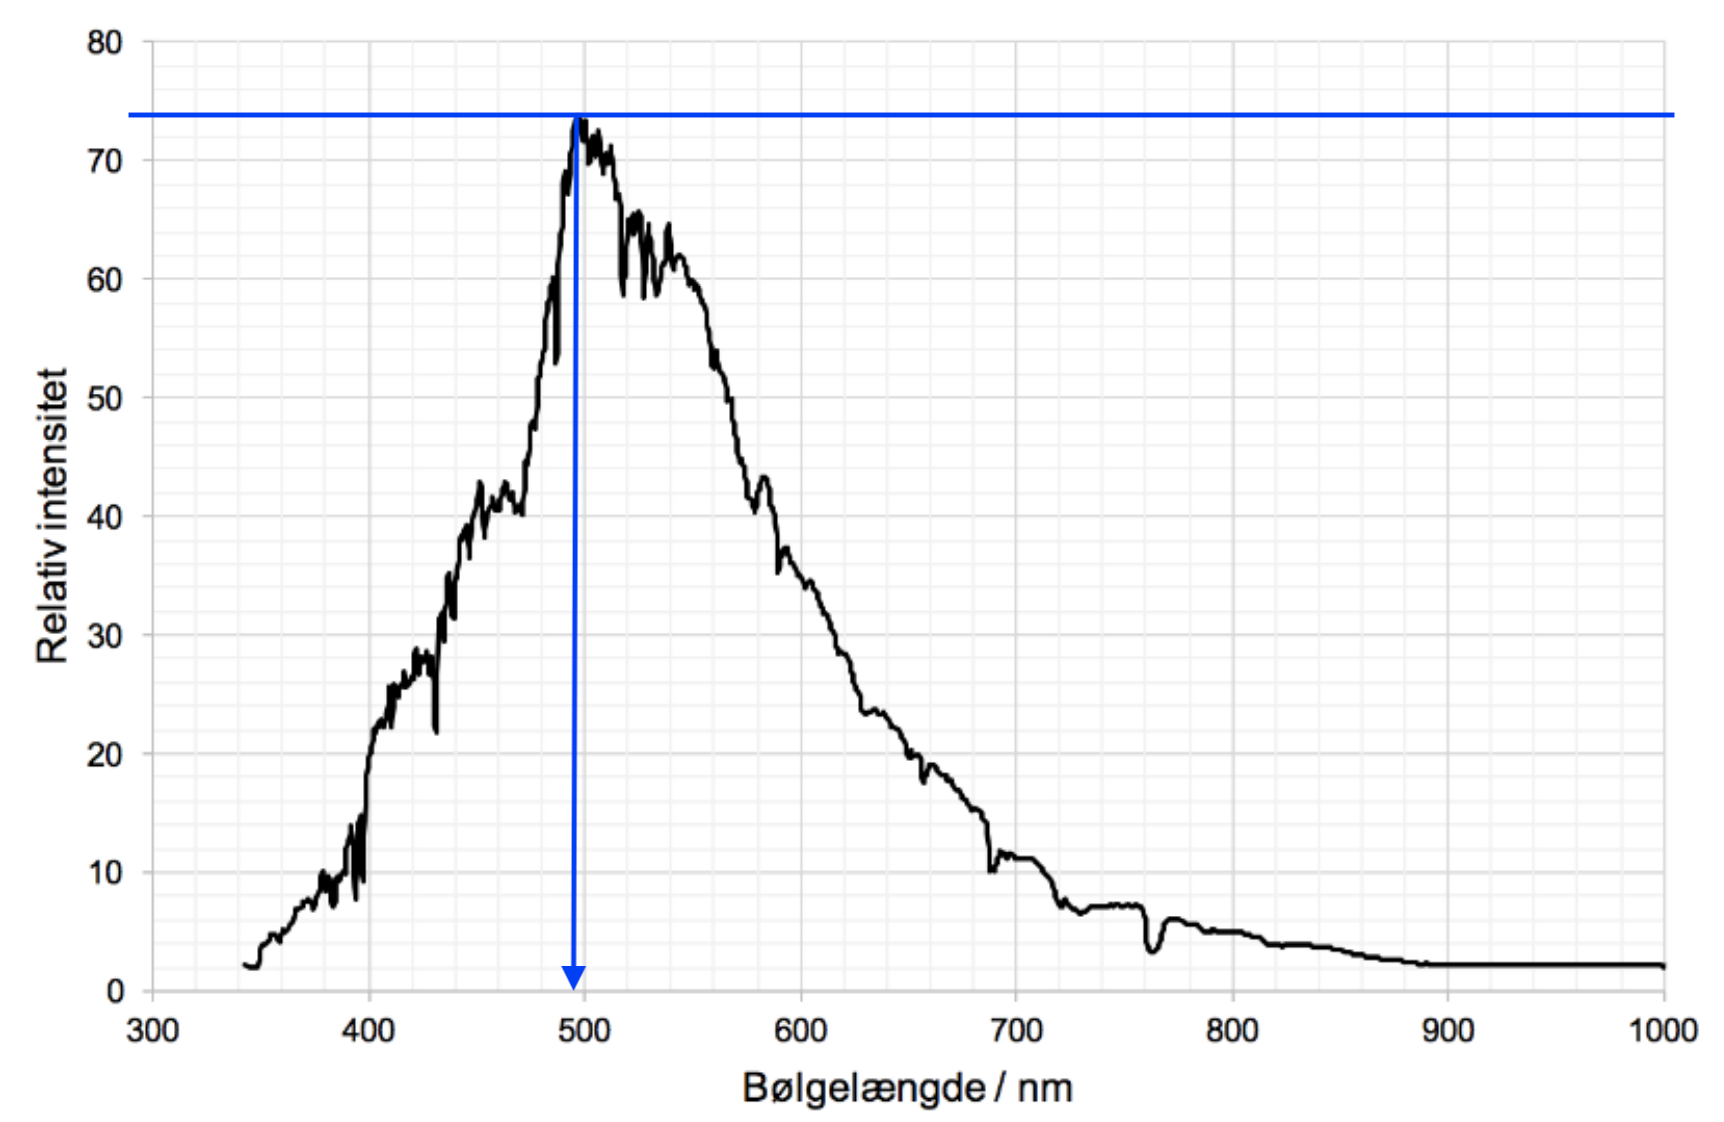
\includegraphics[width=\textwidth]{lys.png}
\end{center}
\caption{Aflæsning på figuren}
\label{fig:lys}
\end{figure}
Energien af en foton med denne bølgelængde må da være
\begin{equation*}
\begin{split}
E _{\text{fot} }&=h \cdot f \\
&=\frac{h \cdot c}{\lambda }\\
&=\frac{6,6261 \cdot 10 ^{-34}\;\unit{J \cdot s} \cdot 3,00 \cdot 10 ^{8} \;\unit{m/s} }{495 \cdot 10 ^{-9}\;\unit{m} }\\
&\approx 4,02 \cdot 10 ^{-19} \;\unit{J} \\
&\approx 2,51 \;\unit{eV} 
\end{split}
\end{equation*}
Energien af en foton med den bølgelængde, hvor lyset har størst relativ intensitet er altså $4,02 \cdot 10 ^{-9}\;\unit{J} $, hvilket svarer til $2,51 \;\unit{eV} $.\\[1ex]
\textbf{b.}
De almindelige briller vil ikke umiddelbart ændre på lysets relative intensitet ved forskellige bølgelængder, og det er da klart, at graf A passer til de almindelige briller.

Grafen, der hører til brillerne med blålysfilter må være som for de almindelige briller, bortset fra, at den relative intensitet må være mindre for en del af bølgelængderne for blåt lys (omkring lidt over $400 \;\unit{nm} $).
Dette må være tilfældet, da de absorberer en del af det blå lys.
Vi ser da, at graf B må passe med brillerne med blålysfilter.

Fra udelukkelsesmetoden har vi så, at graf C må passe med solbrillerne.
Det er i overensstemmelse med, at den relative intensitet af næsten alle bølgelængder tilhørende det synlige lys er mindre ift. de to andre grafer, hvilket bidrager til solbrillernes mørke linser.

Altså passer de almindelige briller med graf A, solbrillerne med graf C og brillerne med blålysfilter med graf B.
\end{document}
